%%%%%%%%%%%%%%%%%%%%%%%%%%%%%%%%%%%%%%%%%
% Original author:
% Linux and Unix Users Group at Virginia Tech Wiki
% (https://vtluug.org/wiki/Example_LaTeX_chem_lab_report)
% Modified by: Hector F. Jimenez S, for the Digital Electronics Laboratory.
% License:
% CC BY-NC-SA 3.0 
%%%%%%%%%%%%%%%%%%%%%%%%%%%%%%%%%%%%%%%%%
%----------------------------------------
%	PACKAGES AND DOCUMENT CONFIGURATIONS
%---------------------------------------
\documentclass[paper=a4, fontsize=12pt]{article} 		% A4 paper and 11pt font size
\usepackage[T1]{fontenc} 								% Use 8-bit encoding that has 256 glyphs
%\usepackage{fourier}		 							% Use the Adobe Utopia font for the document 
\usepackage[spanish,english]{babel}						% Spanish Language, templates uses some sections in english.
\selectlanguage{spanish}								% main language.
\usepackage{subfig}
\usepackage{multirow}
\PassOptionsToPackage{spanish}{babel}
\renewcommand{\figurename}{Figura}						% Force rename of figure.
\renewcommand{\figurename}{Fig.}
\usepackage[figurename=Fig.]{caption}
\usepackage[utf8]{inputenc}								% tildes for spanish language.
\usepackage{amsmath,amsfonts,amsthm} 					% Math packages.
\usepackage{minted}										% For syntax highlighting.
	    \renewcommand\listingscaption{Código}			%rename the source code minted !
\usepackage{float}										% Image will be in the same place as you want.!!! x-/
\usepackage{sectsty} 									% Allows customizing section commands
\allsectionsfont{\centering \normalfont\scshape}	   	% Make all sections centered, the default font and small caps
\usepackage{hyperref}
\hypersetup{											%Setups the false color and borders.
    colorlinks=false,
    pdfborder={0 0 0},
}
\newcommand\fnurl[2]{%									% set a simple and quick footnote command and include url.
\href{#2}{#1}\footnote{\url{#2}}%	
}
\usepackage{graphicx}									% Import easyly images.
\graphicspath{ {./images/} }							% Where to look for the images.
\DeclareGraphicsExtensions{.pdf,.png,.jpg}				% Graphics Extension to be used
\usepackage[notes,backend=biber]{biblatex-chicago}		% Bibliography and references.
\bibliography{biblio}									% bibliography filename.
\usepackage{fancyhdr} 									% Custom headers and footers
\pagestyle{fancyplain} 									% Makes all pages in the document conform to the custom headers and footers
\fancyhead{} 											% No page header
\fancyfoot[L]{} 										% Empty left footer
\fancyfoot[C]{} 										% Empty center footer
\fancyfoot[R]{\thepage} 								% Page numbering for right footer
\renewcommand{\headrulewidth}{0pt} 						% Remove header underlines
\renewcommand{\footrulewidth}{0pt} 						% Remove footer underlines
\setlength{\headheight}{13.6pt} 					    % Customize the height of the header
\numberwithin{equation}{section}						% Number equations within sections (i.e. 1.1, 1.2, 2.1, 2.2 instead of 1, 2, 3, 4)
%\numberwithin{figure}{section} 						% Number figures within sections (i.e. 1.1, 1.2, 2.1, 2.2 instead of 1, 2)
\numberwithin{table}{section} 							% Number tables within sections (i.e. 1.1, 1.2, 2.1, 2.2 instead of 1, 2, 3, 4)
\setlength\parindent{0pt} 								% Removes all indentation from paragraphs
\newcommand{\horrule}[1]{\rule{\linewidth}{#1}} 		% Create horizontal rule command with 1 argument of height
\usepackage{listings}% http://ctan.org/pkg/listings
\usepackage{multicol}
\usepackage{caption}
\usepackage{subfig}
\renewcommand{\lstlistingname}{Código}	
\title{Sistemas Operativos I\\ 
\horrule{0.5pt} \\[0.4cm] 								% Thin top horizontal rule	Title rule
\textit{Taller 6: Caso de estudio del sistema operativo Solaris 10}
\horrule{1pt} \\[0.5cm] 			
} 			

\author{												
Héctor F. \textsc{Jiménez Saldarriaga.}\\				% Authors begin.
\texttt{hfjimenez@utp.edu.co} \\						
\texttt{PGP KEY ID: 0xB05AD7B8}
} 
% End of  Author name
\date{}    						                       % Date for the report, this will hide the \today.

\begin{document}
\maketitle                      			           % Insert the title, author and date
\begin{center}
\begin{tabular}{l r}								   % two column to
Fecha de Entrega: & Marzo, 2018 \\				   % Ramiro's Details.
Profesor: & Cesar Manuel Castillo Rodriguez
\end{tabular}
\end{center}
%%%%%%%%%%%	
% Let's start the document.
%%%%%%%%%%%	
\section{Objetivos}
\begin{itemize}
	\item Evolución
	\item Realizar el proceso de instalación del sistema operativo	
    \item Identificar el manejo de Archivos, Shell
    \item Estructura del Sistema Operativo
    \item Clasificación del Sistema Operativo
	\item Ejecución de Comandos, al menos 20.
\end{itemize}
\section{Evolución de Solaris} 
\section{Proceso de instalación Unix System V R4}
\begin{figure}[H]
 	\centering
   	\subfloat[Bienvenida Instalador Unix System V R4]{\label{fig:bienvenida}{
   		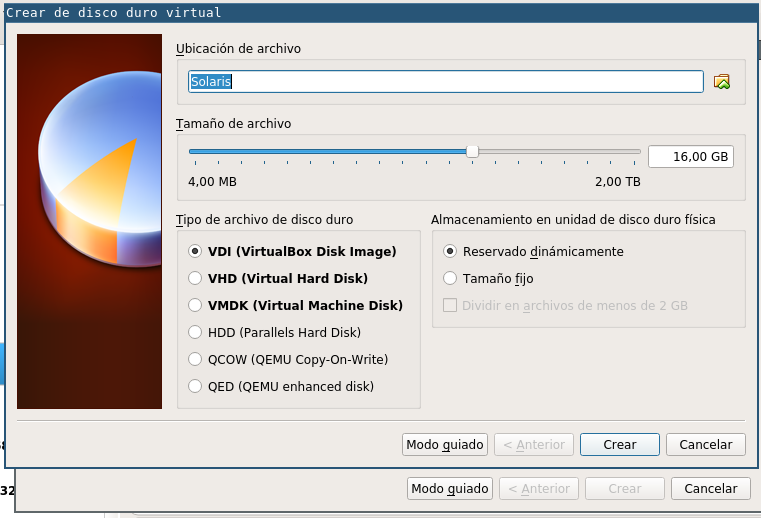
\includegraphics[width=0.68\textwidth]{img/2.png}
   		}}
	\subfloat[Aceptando terminos de instalacion de Unix]{\label{fig:formateada}{
   		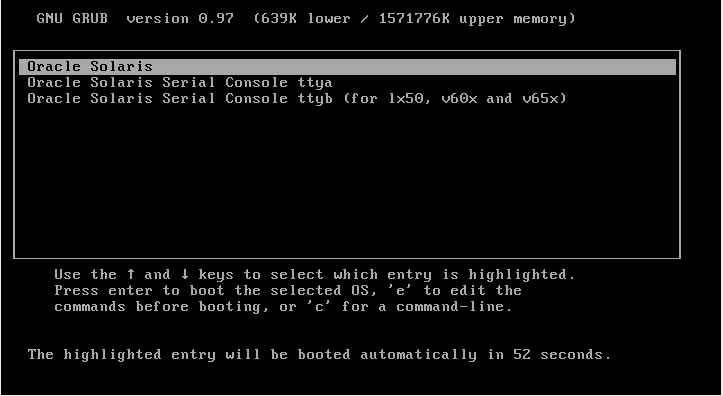
\includegraphics[width=0.68\textwidth]{img/3.png}
        }}
       \hfill
	\subfloat[Utilizaremos 100\% del disco  para la instalacion.]{\label{fig:disco}{
   		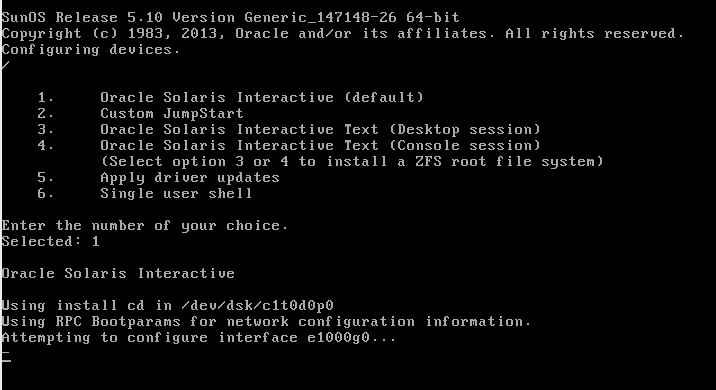
\includegraphics[width=0.68\textwidth]{img/4.png}
        }}
	\subfloat[Seleccion  del Sistema de Archivos para la Instalacion\textit{ufs}]{\label{fig:ufs}{
   		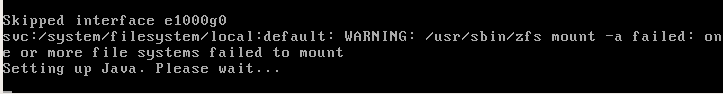
\includegraphics[width=0.68\textwidth]{img/5.png}
        }}
        \hfill
	\subfloat[Confirmación de particiones y ubicación de instalación.]{\label{fig:confirmar}{
   		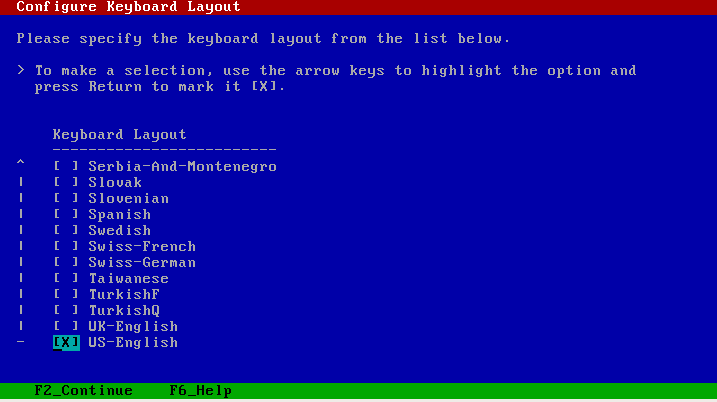
\includegraphics[width=0.68\textwidth]{img/6.png}
        }}
	\subfloat[El sistema decide los tamaños para las particiones.]{\label{fig:particiones}{
   		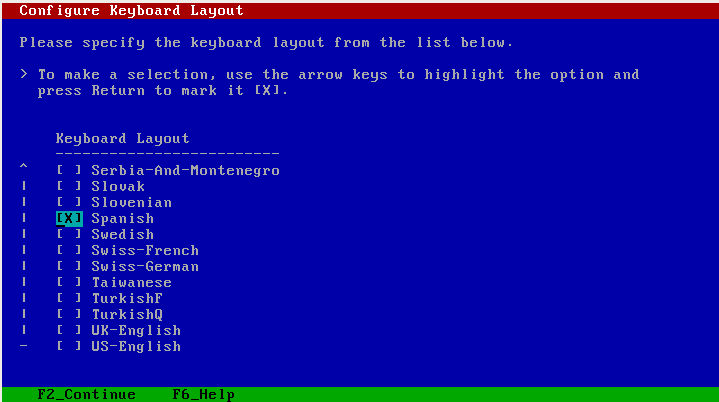
\includegraphics[width=0.68\textwidth]{img/7.png}
        }}
	\caption{Configuración inicial de instalación}
\end{figure}

\begin{figure}[H]
 	\centering
   	\subfloat[]{\label{fig:bienvenida}{
   		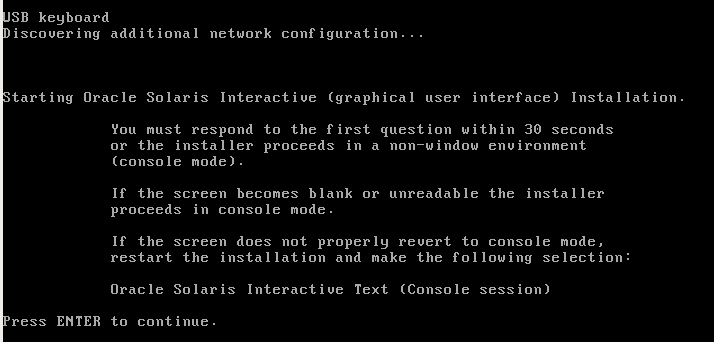
\includegraphics[width=0.68\textwidth]{img/8.png}
   		}}
	\subfloat[]{\label{fig:formateada}{
   		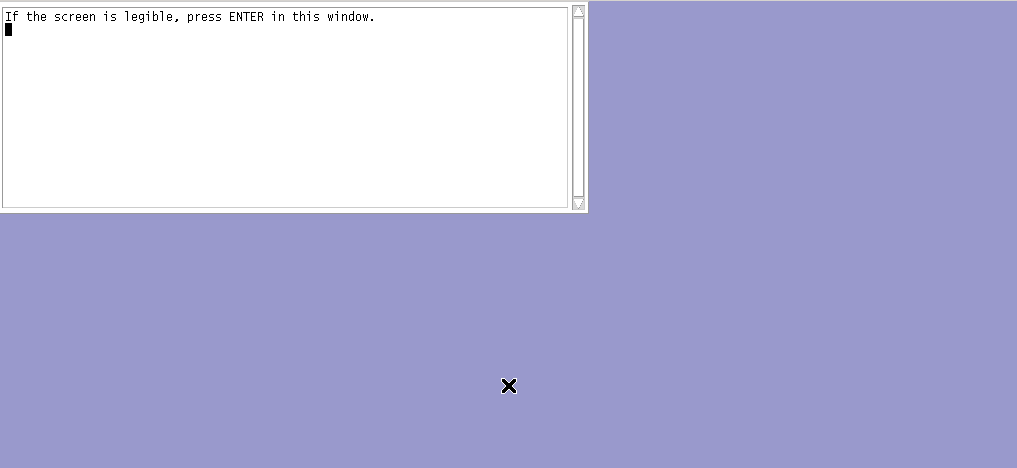
\includegraphics[width=0.68\textwidth]{img/9.png}
        }}
       \hfill
	\subfloat[]{\label{fig:disco}{
   		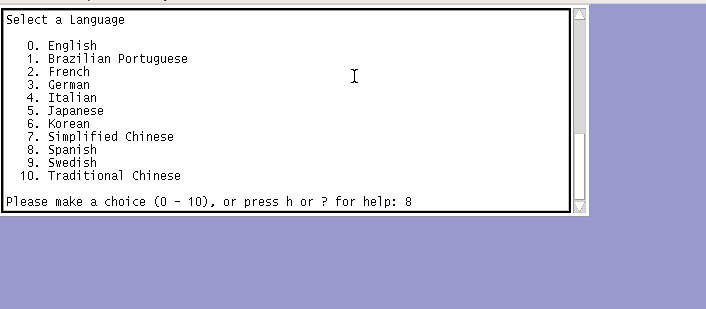
\includegraphics[width=0.68\textwidth]{img/10.png}
        }}
      \subfloat[Ultimo Diskette 10 de 10]{\label{fig:ufs}{
   		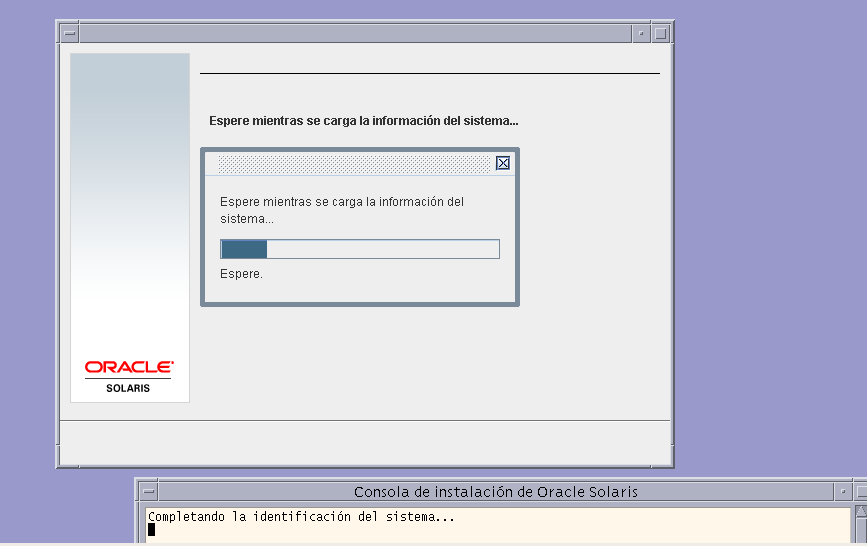
\includegraphics[width=0.68\textwidth]{img/11.png}
        }}
	\caption{Proceso secuencial de instalación, intercambio de diskettes}
\end{figure}

\section{Manejo de Archivos y Estructura}
%Formato imagen unica
%\begin{center}
%\begin{figure}[H]
%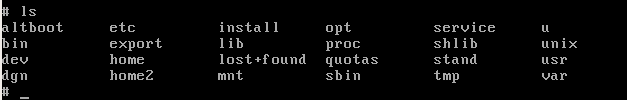
\includegraphics[scale=0.6]{img/directorios.png}
%\caption{Sistema de Archivos Disponible}
%\label{fig:dis2}
%\end{figure}
%\end{center}

\section{Ejecucion Comandos}
\section{Referencias}
%\begin{itemize}
%\item  \hyperref[https://www.youtube.com/watch?v=6P57ukAtCGs&spfreload=10]{Installation of Unix System V on virtualbox Youtube,  https://www.youtube.com/watch?v=6P57ukAtCGs\&spfreload=10}
%\end{itemize}
\end{document}